A block of wood has the shape of a right circular cylinder with radius $6$ and height $8$, and its entire surface has been painted blue. Points $A$ and $B$ are chosen on the edge on one of the circular faces of the cylinder so that the arc ${AB}$ on that face measures $120^\circ$. The block is then sliced in half along the plane that passes through point $A$, point $B$, and the center of the cylinder, revealing a flat, unpainted face on each half. The area of one of those unpainted faces is $a\cdot\pi + b\sqrt{c}$, where $a$, $b$, and $c$ are integers and $c$ is not divisible by the square of any prime. Find $a+b+c$.

\begin{center}
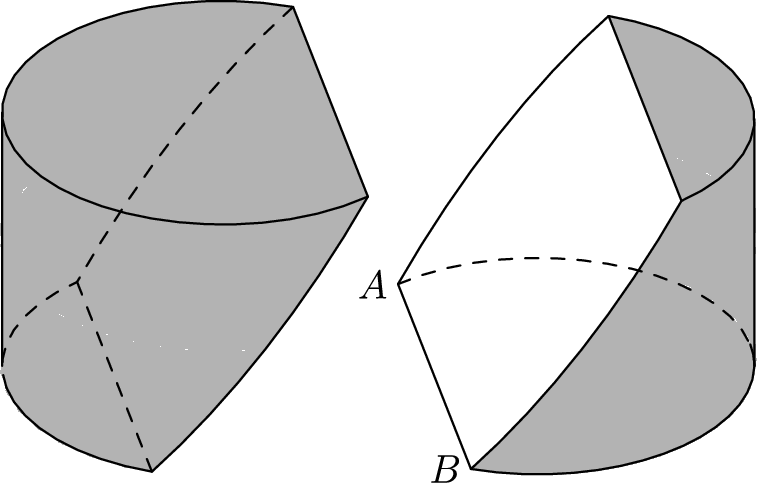
\includegraphics[width = 75.60000000000001mm]{img/fig0.png}
\end{center}
